\documentclass[twoside,twocolumn]{article}

\usepackage{blindtext} 
\usepackage{graphicx}
\usepackage[sc]{mathpazo} 
\usepackage[T1]{fontenc} 
\linespread{1.05} 
\usepackage{microtype} 


\usepackage[english]{babel} 


\usepackage[hmarginratio=1:1,top=32mm,columnsep=20pt]{geometry} 
\usepackage[hang, small,labelfont=bf,up,textfont=it,up]{caption} 
\usepackage{booktabs} 


\usepackage{lettrine} 


\usepackage{enumitem} 
\setlist[itemize]{noitemsep} 


\usepackage{abstract} 
\renewcommand{\abstractnamefont}{\normalfont\bfseries} 
\renewcommand{\abstracttextfont}{\normalfont\small\itshape} 


\usepackage{titlesec} 
\renewcommand\thesection{\Roman{section}} % 
\renewcommand\thesubsection{\roman{subsection}} 
\titleformat{\section}[block]{\large\scshape\centering}{\thesection.}{1em}{} 
\titleformat{\subsection}[block]{\large}{\thesubsection.}{1em}{} 


\usepackage{fancyhdr} 
\pagestyle{fancy} 
\fancyhead{} 
\fancyfoot{} 
\fancyhead[C]{Trabajo de la Unidad I: Proyecto TREVA $\bullet$ Junio 2020 $\bullet$ } 
\fancyfoot[RO,LE]{\thepage} 


\usepackage{titling} 


\usepackage{hyperref} 


%----------------------------------------------------------------------------------------
%	TILULOS
%----------------------------------------------------------------------------------------


\setlength{\droptitle}{-4\baselineskip} 

\pretitle{\begin{center}\Huge\bfseries} 
\posttitle{\end{center}} 
\title{Implementación de Call Center y asistencia para el poder judicial} 
\author{Samuel  - Franklin Carlos, Huichi Contreras, \\
Anthony Robles Flores. }
\date{\today} 
\renewcommand{\maketitlehookd}{
\begin{abstract}
\noindent 
Determino las estrategias que debiera tenerse en cuenta para planificar, estructurar y finalmente escribir un articulo o “paper” de Ciencias Sociales
conforme a la Asociacion Americana de Psicologa (APA) Sexta Edicion. Se pretende que el lector produzca su propio trabajo.
\end{abstract}
\begin{abstract}
\noindent 

Treva es un sistema enfocado en los formularios de satisfacion del cliente en donde el propietario podra generar formularios y enviar cada cierto tiempo a sus empleado o interesados para que puedan llenarlo segun
las opciones que cuenta el formulario, a partir de esos datos podemos al propietario dar estadisticas en la cual puede verificar que opciones escogieron los clientes o empleados, y aparte de ello podemos analizar los datos
para dar recomendaciones o proyecciones estimadas de areas especificas.

\end{abstract}
}

%----------------------------------------------------------------------------------------

\begin{document}

% Print the title
\maketitle

%----------------------------------------------------------------------------------------
%	INTRODUCCION
%----------------------------------------------------------------------------------------

\section{Introduccion}

Los centros de llamada operadas o de contacto  hoy en dia por personal es una proveedora de servicios que se encarga de dar soporte y administrar dependiendo los servicios o solicitudes que las empresas proveen. Estos Centros de contactos normalmente son operados en instalaciones que cuentan con equipos como computadoras, telefonos, microfonos,etc. Estos centros suelen estar conectados con algun otro centro o tambien son prestadoras de servicios de estaciones ya establecidas.\\
Actualmente las mas reconocidas e importantes empresas usan centros de contacto para realizar una interaccion con los clientes entre ellos podemos 
contar firmas para pedidos por catalogo, soportes operativos, atencion al cliente, etc.

\section{Planteamiento del problema}
\subsection{Descripcion del problema}
En el poder judicial se reciben constantes llamadas de parte del publico la cual buscan resolver problema que involucran con la institucion, el problema nace cuando el personal que atiende
el problema no es el calificado para resolverla y este lo redirecciona a otra persona y de esta manera el solicitante se queda buscando a alguien que pueda resolver esta duda haciendo de
esta una experiencia lenta y tediosa.

\subsection{Formulación del problema}
\subsubsection{General}
¿Lograra un call center mediante un asistente virtual resolver las consultas de los clientes ?

\subsection{Justificacion}
El proyecto que a continuación se presenta, no sólo busca responder las consultas del publico solicitante, sino espera lograr,
a través de la tecnología, la automatizacion de consultas extras que puedan ser facilmente contestadas aprovechando el servicio implementado.
La finalidad principal de éste proyecto es aportar una solución tecnológica de corto y largo plazo para un proceso que mejore la atencion al cliente
dentro del Poder Judicial.

\subsection{Alcance}
El alcance final del trabajo será lograr implementar un
software que logre mejorar la atencion de las personas que tengan dudas o consultas acerca del Poder Judicial, siendo estas capaces de responder.

Para solucionar esta problematica existente en el poder judicial tomando en cuenta estos tiempos de la pandemia donde el asilamiento social a provocado un desvalance en las actividades normales de los trabajadores en esta entidad sobrecargando con labores adicionales para el proceso de adaptamiento a este contexto en el que vivimos , la implementacion de un Call Center podria agilizar los procesos de los trabajadores donde un asistente podria solucionar las interrogantes que podrian tener los usuarios antes que un trabajador interno pueda intervenir, pero en caso el asistente no pudiese resolver esta duda , el mismo call center podria derivar a un anexo a poder comunicarse via telefonica con un asesor legal.
\\
Viendo que existen diferentes canales de comunicacion,  en el momento de interactuar con el usuario , proponemos tambien una aplicacion Movil en Android donde este prodra otorgar los mismos servicios añadiendo tambien la facilidad al usuario de poder ubicar las oficinas de acuerdo a la sucursal en la que necesiter asistir a una cita programada , como tambie  el llenado de formularios con formatos ya establecidos por el poder judicial donde hay algunos documetos que no se necesiten la evaluacion de un abogado y como resultado la aplicacion podria descargar un PDF con los datos solicitados usando el formato de documentos del Poder Judicial.
\\
Tomando en cuenta que la tecnologia de tener un SmartPhone invade cada vez mas a la sociedad , incluir un módulo en el aplicativo acerca de las audiencias que el poder judicial publicará asi el usuario externo podría tener a la mano esta información a fin de poder asistir y estar pendientes puesto que en la web se encuentra el cronograma pero ubicar una audiencia para aquellos que desconocen el uso de una plataforma web podria ser dificultoso , la aplicacion movil podria ayudar a que sera mas sencillo y rápido de identificar una audiencia.

\subsection{Tecnologia de informacion}
En esta seccion definiremos las herramientas que se utilizaran para el desarrollo del proyecto asi mismos las plataformas que se emplearan para las conexiones en algunos servicios.
\begin{itemize}
\item Plataforma Colaborativa
\subitem Github
\subitem Google Meet
\subitem Teams Microsoft
\item Base de Datos:
\subitem Firebase.
\item Lenguajes de programación:
\subitem Java.
\item Asistente Virtual:
\subitem DialogFlow.
\item Red Telefonica:
\subitem VoximPlant.

\end{itemize}

\subsection{Metodologia, tecnicas usadas}
La metodologia que usamos para la realizacion es una combinacion de Scrum y Kanban, por el lado de scrum realizamos historias de usuario y el product backlog, como tambien la division de tareas y su estimacion de importancia y tiempo. En medio del sprint usamos kanban para realizar una tabla en la cual se pondria todas las tareas que se realizarian en cada Sprint, haciendo reunionnes en cada oportunidad que tengamos para ir viendo el avanze del proyecto y su continuacion y mejora de ello. Estas tecnicas fueron escogidas por el grupo debido al tiempo que manejabamos y disponiamos en las horas de clase.

\section{Cronograma}
\begin{figure}[htb]
	\begin{center}
		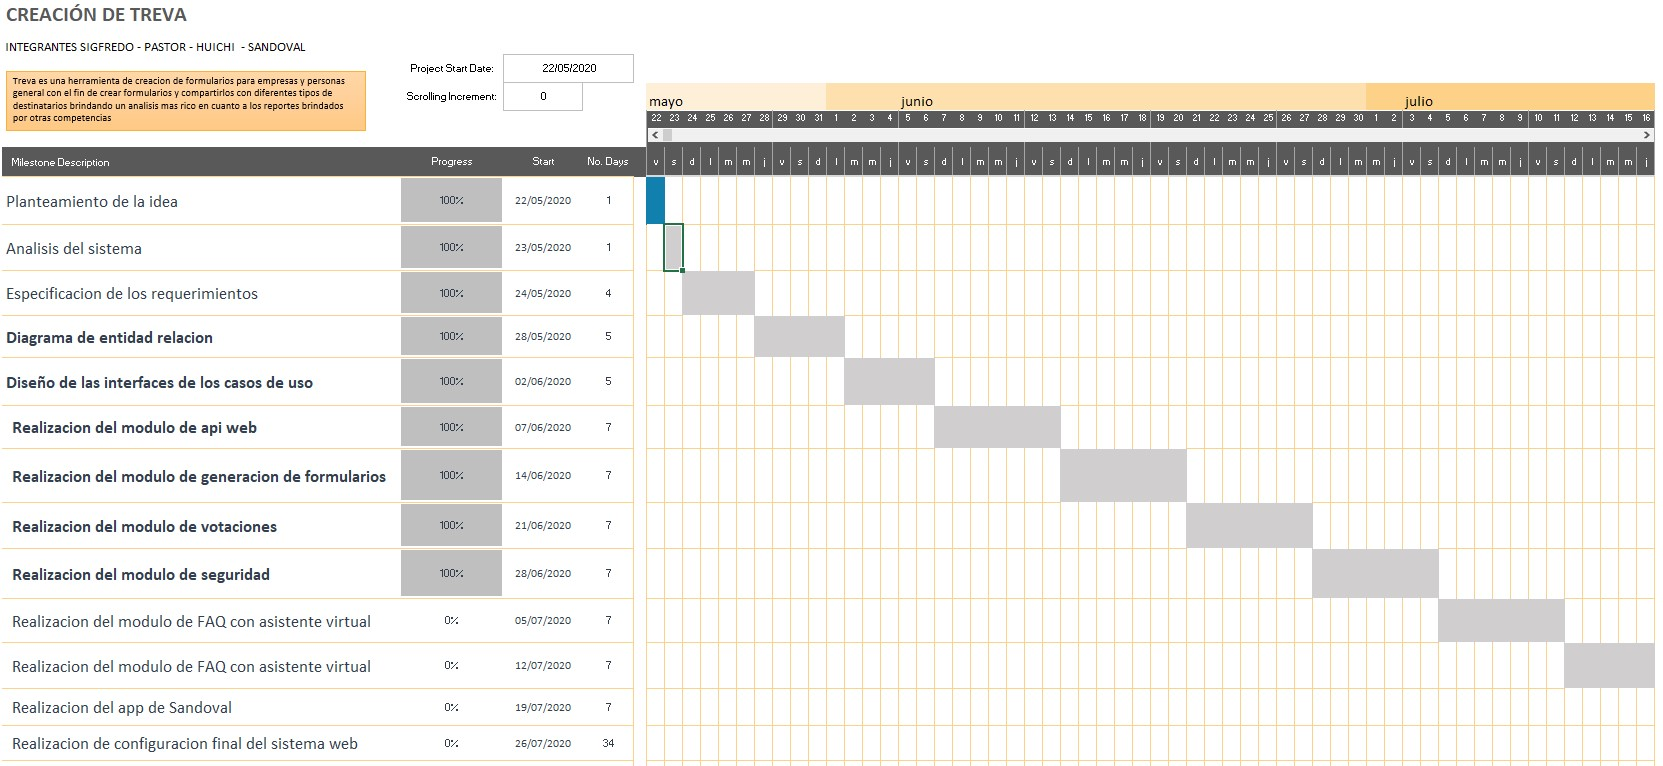
\includegraphics[width=7.5cm]{./Imagenes/Cronograma} 
		\caption{Cronograma}
	\end{center}
\end{figure}


\section{Desarrollo de Solución de Mejora}

\subsection{Casos de Uso de la aplicación}
\begin{figure}[h!]
	\begin{center}
		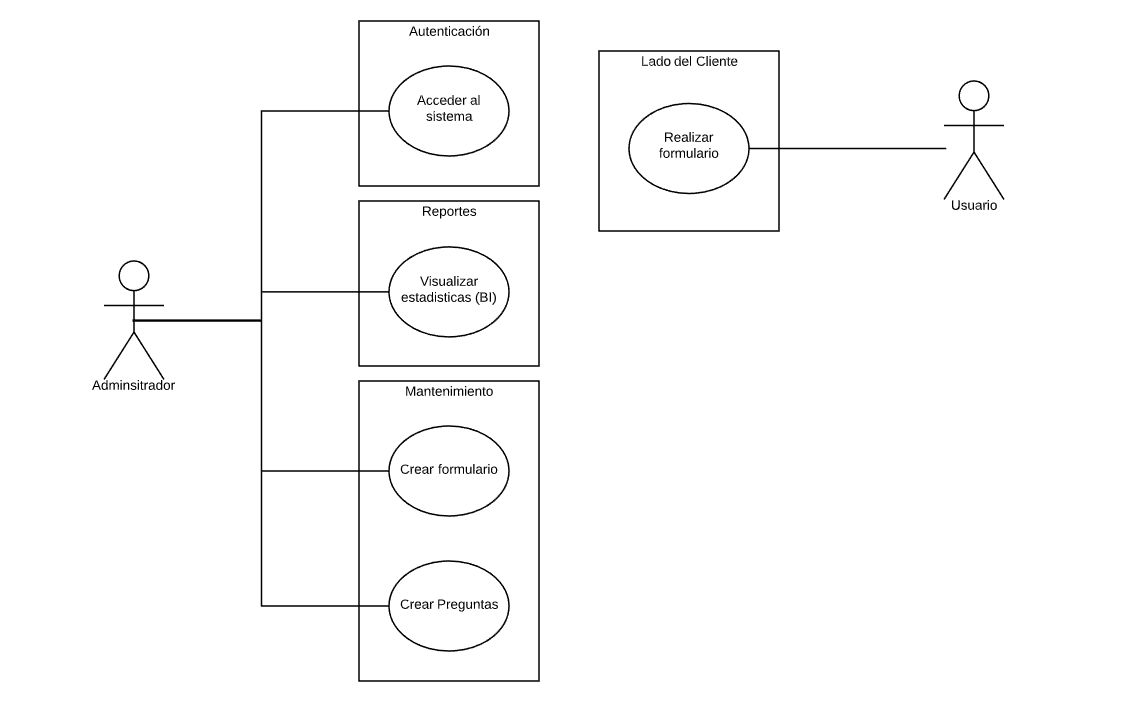
\includegraphics[width=7.5cm]{./Imagenes/use_case} 
		\caption{Use case}
	\end{center}
\end{figure}

\subsection{Diagrama de Arquitectura de la aplicación}
Diagrama de Arquitectura de la aplicación
\begin{figure}[h!]
	\begin{center}
		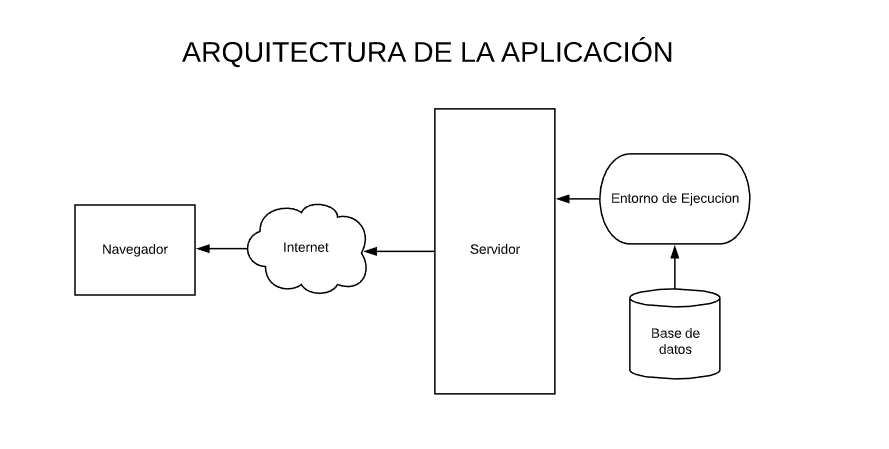
\includegraphics[width=7.5cm]{./Imagenes/bd_architecture} 
		\caption{bd architecture}
	\end{center}
\end{figure}

\subsection{Diagrama de Clases de la aplicación}
Diagrama de Clases de la aplicación
\begin{figure}[h!]
	\begin{center}
		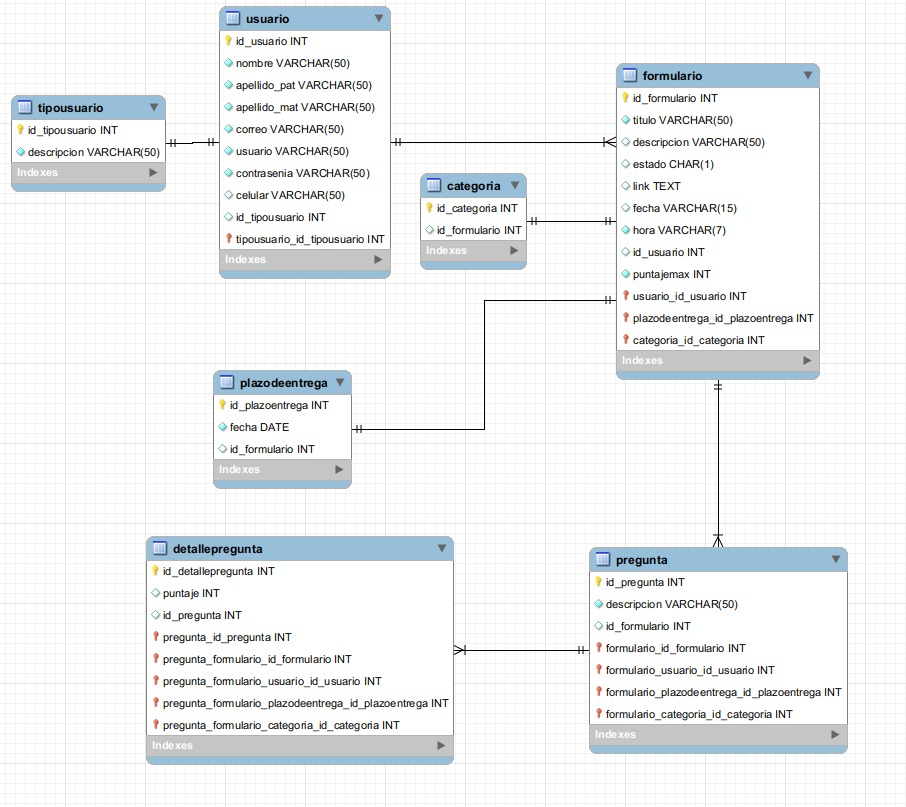
\includegraphics[width=7.5cm]{./Imagenes/diagramclass} 
		\caption{Diagram Class}
	\end{center}
\end{figure}



\end{document}
